%\documentclass[english, times, mirror]{revdetua}
% use this if you're writing in portuguese:
\documentclass[portuguese, times, mirror]{revdetua}

\usepackage[utf8]{inputenc}
\usepackage{graphicx}
\usepackage{hyperref}

\usepackage{amsmath}
\usepackage{mathtools}

\usepackage{caption}
\usepackage{listings}
\usepackage{color}

\definecolor{dkgreen}{rgb}{0,0.6,0}
\definecolor{gray}{rgb}{0.5,0.5,0.5}
\definecolor{mauve}{rgb}{0.58,0,0.82}

\lstset{frame=tb,
  language=Java,    
  aboveskip=3mm,
  belowskip=3mm,
  showstringspaces=false,
  columns=flexible,
  basicstyle={\small\ttfamily},
  numbers=none,
  numberstyle=\tiny\color{gray},
  keywordstyle=\color{blue},
  commentstyle=\color{dkgreen},
  stringstyle=\color{mauve},
  breaklines=true,
  breakatwhitespace=true,
  tabsize=3
}

\usepackage{tikz}
\usepackage{pgfplots}

% correct bad hyphenation here
\hyphenation{op-tical net-works semi-conduc-tor}

\begin{document}

\Header{1}{1}{Setembro}{2016}{1}
% Note: the month must be in Portuguese

\title{Visão por Computador 2016-17, Guia Prático N.º 2}
\author{Rui Oliveira, Tomás Rodrigues\\ DETI, Universidade de Aveiro \\ Aveiro, Portugal \\ \{ruipedrooliveira, tomasrodrigues\}@ua.pt}
% you should be able to use the \and keyword, but the deti format doesn't like it, for some reason
\maketitle

\begin{resumo}


Pretende-se através deste relatório expor sob forma escrita, o nosso desempenho e objetivos alcançados na aula prática n.2 da unidade curricular de Visão por Computador do Mestrado Integrado de Engenharia de Computadores e Telemática.

Neste relatório pretenderemos explicar as soluções por nós encontradas para a resolução dos diferentes problemas propostos.


\end{resumo} 

\begin{palavraschave} %
visão, computador, imagem digital, opencv, c++, 
 \end{palavraschave} %




\section{Repositório: código fonte}


Todas as soluções dos problemas propostos estão disponível através do seguinte repositório (gitHub) criado para o efeito. \\

\href{http://github.com/toomyy94/CV1617-68779-68129}{http://github.com/toomyy94/CV1617-68779-68129}
\\


A resolução dos problemas do presente guia encontram-se na pasta aula2. 



\section{Problemas propostos}



\subsection{Problema \#1 a \#3}

\begin{itemize}
    \item Sistema operativo: Linux
    \item Instalação openCV: https://github.com/jayrambhia/Install-OpenCV
    \item IDE Code::Blocks (http://www.codeblocks.org/downloads)
\end{itemize}

\subsection{Problema \#4}

\subsubsection{Enunciado}
\textit{ Implement, compile and test the OpenCV example “Load, Modify, and Save an Image”.}

\subsubsection{Resolução e principais conclusões}


\begin{itemize}
    \item Carregar imagem: usar método \texttt{imread()} especificando o tipo pretendido 
    \item Aplicar modificação a uma imagem: foram utilizados os métodos \texttt{cvtColor} e \texttt{threshold}.   
    \item Guardar imagem: foi usado o método \texttt{imwrite} especificando o caminho de destino. 
\end{itemize}


\begin{lstlisting}[caption=Proposta de resolução do exercício 4,label=code:C]
    Mat img = imread("../images/lena.jpg", CV_LOAD_IMAGE_COLOR);
    
    if(img.empty())
       return -1;
    cvtColor( img, img, CV_BGR2GRAY );
    threshold(img, img, 100, 255, THRESH_BINARY);
    imwrite( "../images/lena_bin.jpg", img );
    imshow("lena_bin", img);
\end{lstlisting}



\begin{figure}[ht!]
\centering
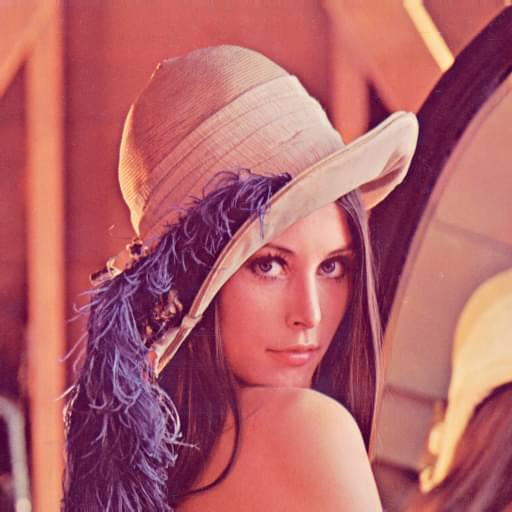
\includegraphics[width=70mm]{img/lena.jpg}
\caption{Imagem original lena.jpp}
\end{figure}



\begin{figure}[ht!]
\centering
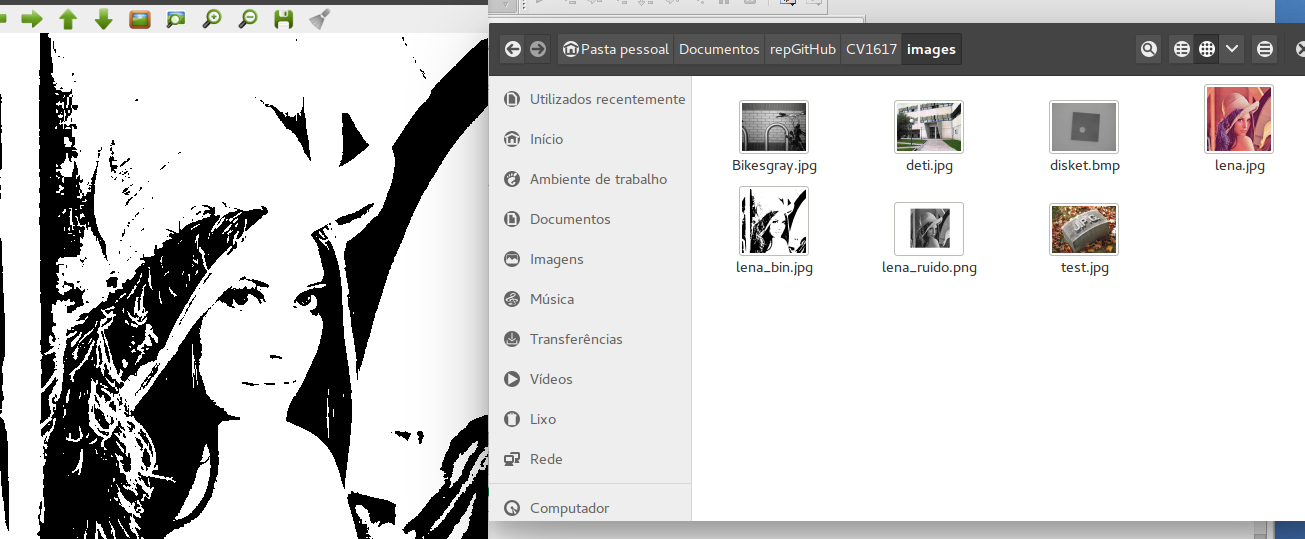
\includegraphics[width=70mm]{img/ex1.png}
\caption{A simple caption \label{overflow}}
\end{figure}


Alternativas também aplicadas neste problema: 

Carregar imagem, aplicar uma conversão para escala de cinza e guardar a imagem. 
\begin{lstlisting}
cvtColor( img, gray_image, CV_BGR2GRAY );
\end{lstlisting}

Carregar imagem, aplicar uma conversão para escala de YUV\footnote{https://en.wikipedia.org/wiki/YUV}  e guardar a imagem. 

\begin{lstlisting}
cvtColor( img, yuv_image, CV_BGR2YUV );
\end{lstlisting}




%%%%%%%%%%%%%%%%%%%%%%%%
\subsection{Problema \#5}

\subsubsection{Enunciado}
\textit{ Implement, compile and test the OpenCV example 'Adding two images using OpenCV'}

\subsubsection{Resolução e principais conclusões}

\begin{itemize}
    \item Foi utilizado o método \texttt{addWeighted()} em que temos os seguintes argumentos:
    \begin{itemize}
        \item \texttt{src1} : ..
        \item \texttt{alpha} : ..
        \item \texttt{src2} : ..
        \item \texttt{beta} :..
        \item \texttt{dst} : ..
    \end{itemize}
    
    
    
\end{itemize}





\begin{lstlisting}[caption=Proposta de resolução do exercício 5,label=code:C]
    double alpha = 0.5; double beta; double input;
    Mat src1, src2, dst;
    namedWindow("Linear Blend", 1);
    beta = ( 1.0 - alpha );
    addWeighted( src1, alpha, src2, beta, 0.0, dst);
    imshow( "Linear Blend", dst );
    waitKey(0);
\end{lstlisting}


Com alpha igual 0.5 o resultado da imagem anterior é a seguinte
\begin{figure}[ht!]
\centering
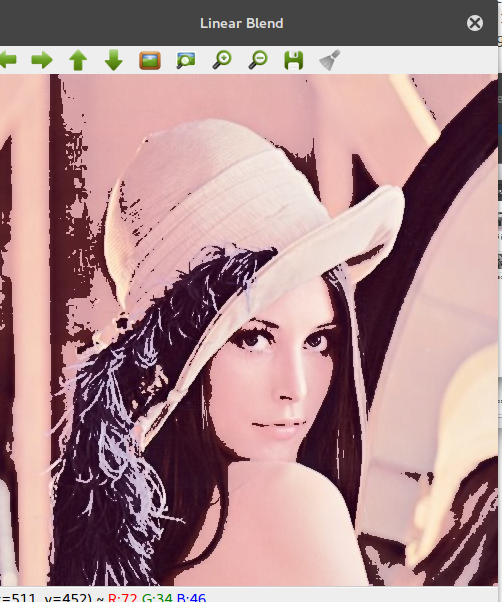
\includegraphics[width=70mm]{img/ex2.png}
\caption{A simple caption \label{overflow}}
\end{figure}




%%%%%%%%%%%%%%%%%%%%%%%%
\subsection{Problema \#6}

\subsubsection{Enunciado}
\textit{ Implement, compile and test the OpenCV example 'Changing the contrast and brightness of an image'.}

\subsubsection{Resolução e principais conclusões}




\begin{lstlisting}[caption=Proposta de resolução do exercício 6,label=code:C]
    double alpha; int beta;
    Mat img = imread("../images/lena.jpg", CV_LOAD_IMAGE_COLOR);
    Mat new_image = Mat::zeros( img.size(), img.type() );
    
    for( int y = 0; y < img.rows; y++ ){
        for( int x = 0; x < img.cols; x++ ){
            for( int c = 0; c < 3; c++ ){
                new_image.at<Vec3b>(y,x)[c] = saturate_cast<uchar>( alpha*( img.at<Vec3b>(y,x)[c] ) + beta );
            }
        }
    }
    
\end{lstlisting}


%%%%%%%%%%%%%%%%%%%%%%%%
\subsection{Problema \#7}

\subsubsection{Enunciado}
\textit{ Change the previous example in order to explore other methods of scanning an image.}

\subsubsection{Resolução e principais conclusões}




\begin{thebibliography}{1} % 9



\bibitem{fsound}
Neves, A. J. R.; Dias, P. Slides teóricos Visão por Computador - Aula 2 (2016)


\bibitem{vtk}
OpenCV. \href{hhttp://docs.opencv.org/}{Opencv Documentation}. Web. 24 Outubro 2016. 




\end{thebibliography}

\end{document}
